\documentclass[10pt]{article}

%%%%%%%%%%%%%%Include Packages%%%%%%%%%%%%%%%%%%%%%%%%%%
\usepackage{xcolor}
\usepackage{mathtools}
\usepackage[legalpaper, margin=1in]{geometry}
\usepackage{amsmath}
\usepackage{amssymb}
\usepackage{paralist}
\usepackage{rsfso}
\usepackage{amsthm}
\usepackage{wasysym}
\usepackage[inline]{enumitem}   
\usepackage{hyperref}
\usepackage{tocloft}
%%%%%%%%%%%%%%%%%%%%%%%%%%%%%%%%%%%%%%%%%%%%%%%%%%%%%%%%

%%%%%%%%%%%%%%%%%Theorem environments%%%%%%%%%%%%%%%%%%%
\newtheoremstyle{break}
  {\topsep}{\topsep}%
  {\itshape}{}%
  {\bfseries}{}%
  {\newline}{}%
\theoremstyle{break}
\theoremstyle{break}
\newtheorem{axiom}{Axiom}
\newtheorem{thm}{Theorem}[section]
\newtheorem{lem}{Lemma}[thm]
\newtheorem{prop}[thm]{Proposition}
\newtheorem{corL}{Corollary}[lem]
\newtheorem{corT}[lem]{Corollary}
\newtheorem{defn}{Definition}[corL]
\newenvironment{indEnv}[1][Proof]
  {\proof[#1]\leftskip=1cm\rightskip=1cm}
  {\endproof}
%%%%%%%%%%%%%%%%%%%%%%%%%%%%%%%%%%%%%%%%%%%%%%%%%%%%%%

%%%%%%%%%%%%%%%%%%%%%%%Integral%%%%%%%%%%%%%%%%%%%%%%%
\def\upint{\mathchoice%
    {\mkern13mu\overline{\vphantom{\intop}\mkern7mu}\mkern-20mu}%
    {\mkern7mu\overline{\vphantom{\intop}\mkern7mu}\mkern-14mu}%
    {\mkern7mu\overline{\vphantom{\intop}\mkern7mu}\mkern-14mu}%
    {\mkern7mu\overline{\vphantom{\intop}\mkern7mu}\mkern-14mu}%
  \int}
\def\lowint{\mkern3mu\underline{\vphantom{\intop}\mkern7mu}\mkern-10mu\int}
%%%%%%%%%%%%%%%%%%%%%%%%%%%%%%%%%%%%%%%%%%%%%%%%%%%%%%



\newcommand{\R}{\mathbb{R}}
\newcommand{\N}{\mathbb{N}}
\newcommand{\Z}{\mathbb{Z}}
\newcommand{\Q}{\mathbb{Q}}
\newcommand{\A}{\mathcal{A}}
\newcommand{\D}{\mathcal{D}}
\newcommand{\J}{\mathcal{J}}
\newcommand{\T}{\mathcal{T}}
\newcommand{\Td}{\mathcal{T}_d}
\newcommand{\C}{\mathcal{C}}
\newcommand{\M}{\mathcal{M}}
\newcommand{\Complex}{\mathbb{C}}
\newcommand{\Power}{\mathcal{P}}
\newcommand{\ee}{\cdot 10}
\newcommand{\spa}{\text{span}}
\newcommand{\vmat}[1]{\begin{vmatrix} #1 \end{vmatrix}}
\newcommand{\rref}{\xrightarrow{\text{row\ reduce}}}


\newcommand{\note}{\color{red}Note: \color{black}}
\newcommand{\remark}{\color{blue}Remark: \color{black}}
\newcommand{\example}{\color{green}Example: \color{black}}
\newcommand{\exercise}{\color{green}Exercise: \color{black}}




%%%%%%%%%%%%table of contents%%%%%%%%%%%%%%%%%%%%%%%%%%%%
\cftsetindents{section}{0em}{2em}
\cftsetindents{subsection}{0em}{2em}

\renewcommand\cfttoctitlefont{\hfill\Large\bfseries}
\renewcommand\cftaftertoctitle{\hfill\mbox{}}

\setcounter{tocdepth}{2}
%%%%%%%%%%%%%%%%%%%%%%%%%%%%%%%%%%%%%%%%%%%%%%%%%%%%%%%%%


%%%%%%%%%%%%%%%%%%%%%Footnotes%%%%%%%%%%%%%%%%%%%%%%%%%%%
\newcommand\blfootnote[1]{%
  \begingroup
  \renewcommand\thefootnote{}\footnote{#1}%
  \addtocounter{footnote}{-1}%
  \endgroup
}
%%%%%%%%%%%%%%%%%%%%%%%%%%%%%%%%%%%%%%%%%%%%%%%%%%%%%%%%%

\makeatletter
\def\@seccntformat#1{%
  \expandafter\ifx\csname c@#1\endcsname\c@section\else
  \csname the#1\endcsname\quad
  \fi}
\makeatother


%%%%%%%%%%%%%%%%%%%%%%%%%%%%%%%%%%%Enumerate%%%%%%%%%%%%%%
\makeatletter
% This command ignores the optional argument 
% for itemize and enumerate lists
\newcommand{\inlineitem}[1][]{%
\ifnum\enit@type=\tw@
    {\descriptionlabel{#1}}
  \hspace{\labelsep}%
\else
  \ifnum\enit@type=\z@
       \refstepcounter{\@listctr}\fi
    \quad\@itemlabel\hspace{\labelsep}%
\fi}
\makeatother
\parindent=0pt
%%%%%%%%%%%%%%%%%%%%%%%%%%%%%%%%%%%%%%%%%%%%%%%%%%%%%%%%%%


\begin{document}
For adiabatic process, $T_iV_i^{\gamma-1}= T_fV_f^{\gamma-1}$, where $\gamma = C_p / C_v$. Alternatively, we write $p_iV_i^{\gamma} = p_fV_f^{\gamma}$.\\

Otto cycle consists of two isobaric processes on the sides, and adiabatic processes on top and bottom.\\

For an engine, $Q_H>0$ is the heat get into the system, $Q_C<0$ is the heat goes out of the system. $W>0$ is the work done by the engine. $|Q_H| = |W| + |Q_C|$. Efficiency of an engine is given by:$$e = 1+\frac{Q_C}{Q_H} = \frac{|W|}{|Q_H|}$$ 

For Otto cycle, we have $e = 1- \frac{1}{r^{\gamma-1}}$.\\
For Carnot cycle, we have $e = 1 - \frac{T_C}{T_H}$, which is the most efficient engine.\\

For refrigerator, $Q_C>0$ is the heat removed from the cold region and enter the system, $W<0$ is the work done by the surroundings to the system, and $Q_H < 0$ is the heat that leaves the system as part of the cooling process. The coefficient of performance of the refrigerator is given by: $$K = \frac{|Q_C|}{|W|} = \frac{|Q_C|}{|Q_H| - |Q_C|}$$

\textbf{Second Law of Thermodynamics}:\\
(1) It is impossible for any process to have its sole result the transfer of heat from a cooler to a hotter body.\\
(2) it is impossible for any system
to undergo a process in which it absorbs heat from a reservoir at a single temperature and converts the heat completely into mechanical work, with the system ending in the same state as it begins. There is no $100\%$ efficient engine.\\
(3) The change in entropy of the entire system is always greater than or equal to zero in all
physical processes.\\
The Second Law of Thermodynamics express the one-way aspect of thermodynamic process:
organized becomes more disorganized.\\

The infinitesimal change in entropy, denoted as $dS$, in an infinitesimal reversible process at absolute temperature T is given by $dS =
\frac{dQ}{T}$. For isothermal process, we have: $$\Delta S = \int_i^f \frac{dQ}{T} = \frac{\Delta Q}{T} = nR\ln(\frac{V_b}{V_a})$$ $[S] = J/K$. The change in entropy is path independent, for cyclic process, change in entropy is $0$.\\

Let $M_{\C}$ be the number of microstates in macrostate $\C$. Then entropy of the macrostate is given by $S_{\C} = k\ln(M_{\C})$, where $k = 1.38064852\cdot 10^{-23}\ \frac{m^2\, kg}{s^2 K}$ is the Boltzmann's constant. $\Delta S = k\ln (M_f/M_i)$. \\

Clausius' Inequality: $\Delta S \geq \int \frac{dQ}{T}$ for non-reversible processes, and equality holds for reversible processes.\\

Wave equation $\frac{\partial^2 y}{\partial x^2}= \frac{1}{v^2} \frac{\partial^2 y}{\partial t^2}$ has a solution $y = A\cos(kx\pm \omega t)$, with $v = \omega / k = \lambda f \Rightarrow k=2\pi/\lambda$.\\

A string with uniform mass density $\mu$, average power in one wavelength of the wave carried by the string is given by $P_{avg}$. Let $\omega$ be the angular frequency, $A$ be the amplitude of the wave, and $v$ be
the speed of the wave. Suppose further that the string has tension $T$, we write the following:
$$P_{avg} = \frac{1}{2}\mu \omega^2 A^2 v\qquad\qquad \qquad v = \sqrt{\frac{T}{\mu}}\qquad\qquad\Rightarrow\qquad \qquad P_{avg} = \frac{1}{2}\sqrt{\mu T}\omega^2 A^2$$

Superposition principle states that if two waves have the same speed, then the sum of the two waves is also a solution to the same wave equation. \\

The direction of propagation of an EM wave is given by $\vec{E}\times \vec{B}$. \\
$$\frac{\partial^2 B}{\partial x} - \frac{1}{c^2}\frac{\partial^2 B}{\partial t^2} = 0\qquad\qquad\qquad  c = \sqrt{1/(\mu_0 \epsilon_0)}\qquad\qquad\qquad B_{max}=\frac{E_{max}}{c}$$

$$\vec{S} = \frac{1}{\mu_0}\vec{E}\times \vec{B}\qquad\qquad S_{avg} = I = \frac{1}{\mu_0 c}E_{max}^2=\frac{1}{2}\epsilon_0 c E_{max}^2 = \frac{Power}{Area}$$

$$u_E = \frac{1}{2}\epsilon_0 E_{avg}^2 \qquad\qquad u_B = \frac{1}{2}\frac{B_{avg}^2}{\mu_0}\qquad\qquad E_{avg}^2 = E_{max}^2/2\qquad\qquad B_{avg}^2 = B_{max}^2/2$$

If the wave is totally absorbed, $\text{Momentum in EM wave} = \frac{S_{avg}}{c}$. \\If the wave is totally reflected, $\text{Momentum in EM wave} = \frac{2S_{avg}}{c}$.\\

Index of refraction of a material is given by $n = c/b$.

\textbf{Laws of Reflection and Refraction}:\\
(1) The incident ray, reflected ray, and refracted ray all lie in the same plane, called the plane of incidence.\\
(2) The degree of incident angle is equal to the degree of reflection angle.\\
(3) Snell's Law holds: $n_a \sin(\theta_a) = n_b\sin(\theta_b)$.\\

Typically, index of refraction is smaller for light of larger wavelengths, and larger for light of shorter wavelengths, so red light would typically has smaller index of refraction than the blue light does. 

\newpage
There are two coherent sources, consider a point $p$, with distance $r_1$ from one of the source, and $r_2$ from the other source. Let $m \in \Z$ be arbitrary.\\
Constructive interference happens when $r_2 - r_1 = m\lambda$. \\
Destructive interference happens when $r_2 - r_1 = (m+\frac{1}{2})\lambda$. \\

Suppose a string has length $L$, then the standing wave on the string have modes characterized by:
$$\lambda_n = \frac{2L}{n} \qquad\qquad f_n =\frac{v}{\lambda_n}= \frac{v}{2L}\cdot n$$
$f_1 = \frac{v}{2L}$ is called the fundamental frequency. $f_{n} = n f_1$ is the $(n-1)$-th overtone, or the $n$-th harmonic. \\

For interference in the \textbf{double}-slit experiment:
$$I = I_0 \cos^2\left(\pi \frac{d}{\lambda} \sin(\theta)\right)\qquad\qquad\qquad I_0 = 2\epsilon_0 c E_0^2$$
where $E_0$ is the amplitude of the Electric field of the wave coming out from one of the two slits. \\

For diffraction of light in a \textbf{single}-slit:
$$I = I_0 \left(\frac{\sin(\beta/2)}{\beta/2} \right)^2 \qquad\qquad \beta = 2\pi\frac{a}{\lambda} \sin(\theta)$$
where $a$ is the width of the slit.\\

Combing diffraction and interference in the \textbf{double}-slit experiment:
$$I = I_0 \left(\frac{\sin(\beta/2)}{\beta/2} \right)^2 \cos^2\left(\pi \frac{d}{\lambda} \sin(\theta)\right)$$
\hfill\break
\begin{center}
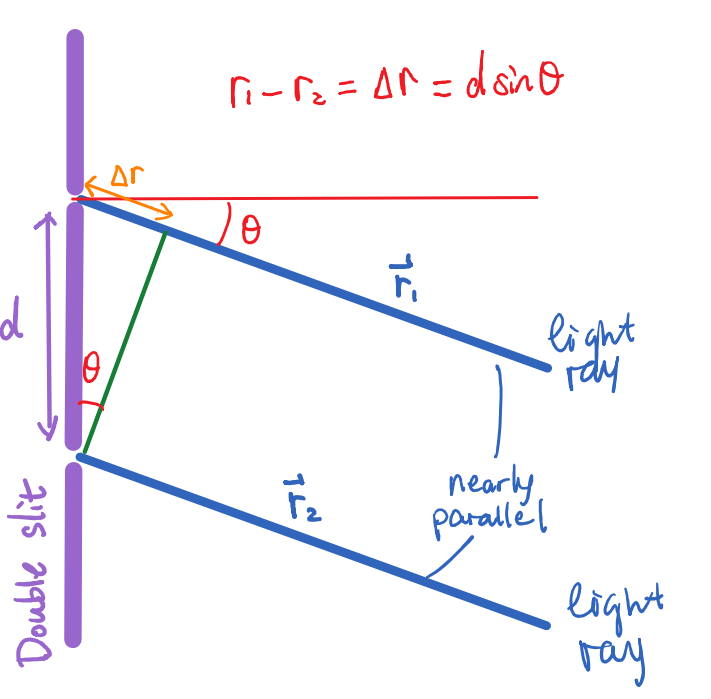
\includegraphics[scale=0.3]{slits.png}\qquad\qquad\qquad
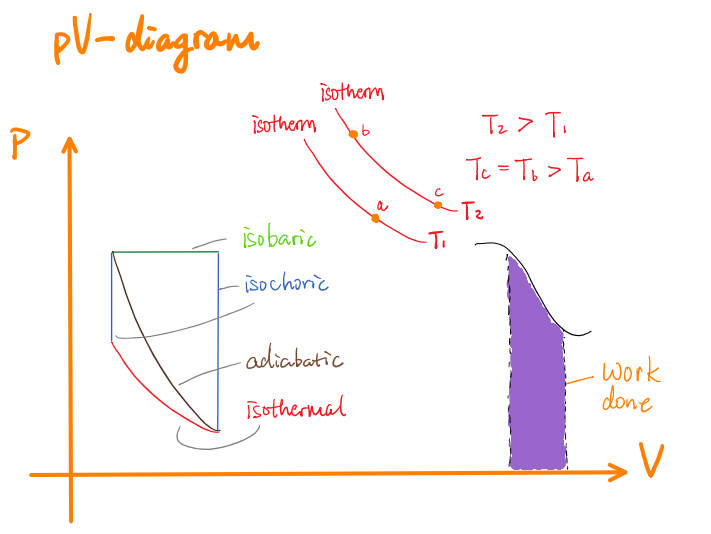
\includegraphics[scale=0.39]{thermo.png}
\end{center}


\begin{center}
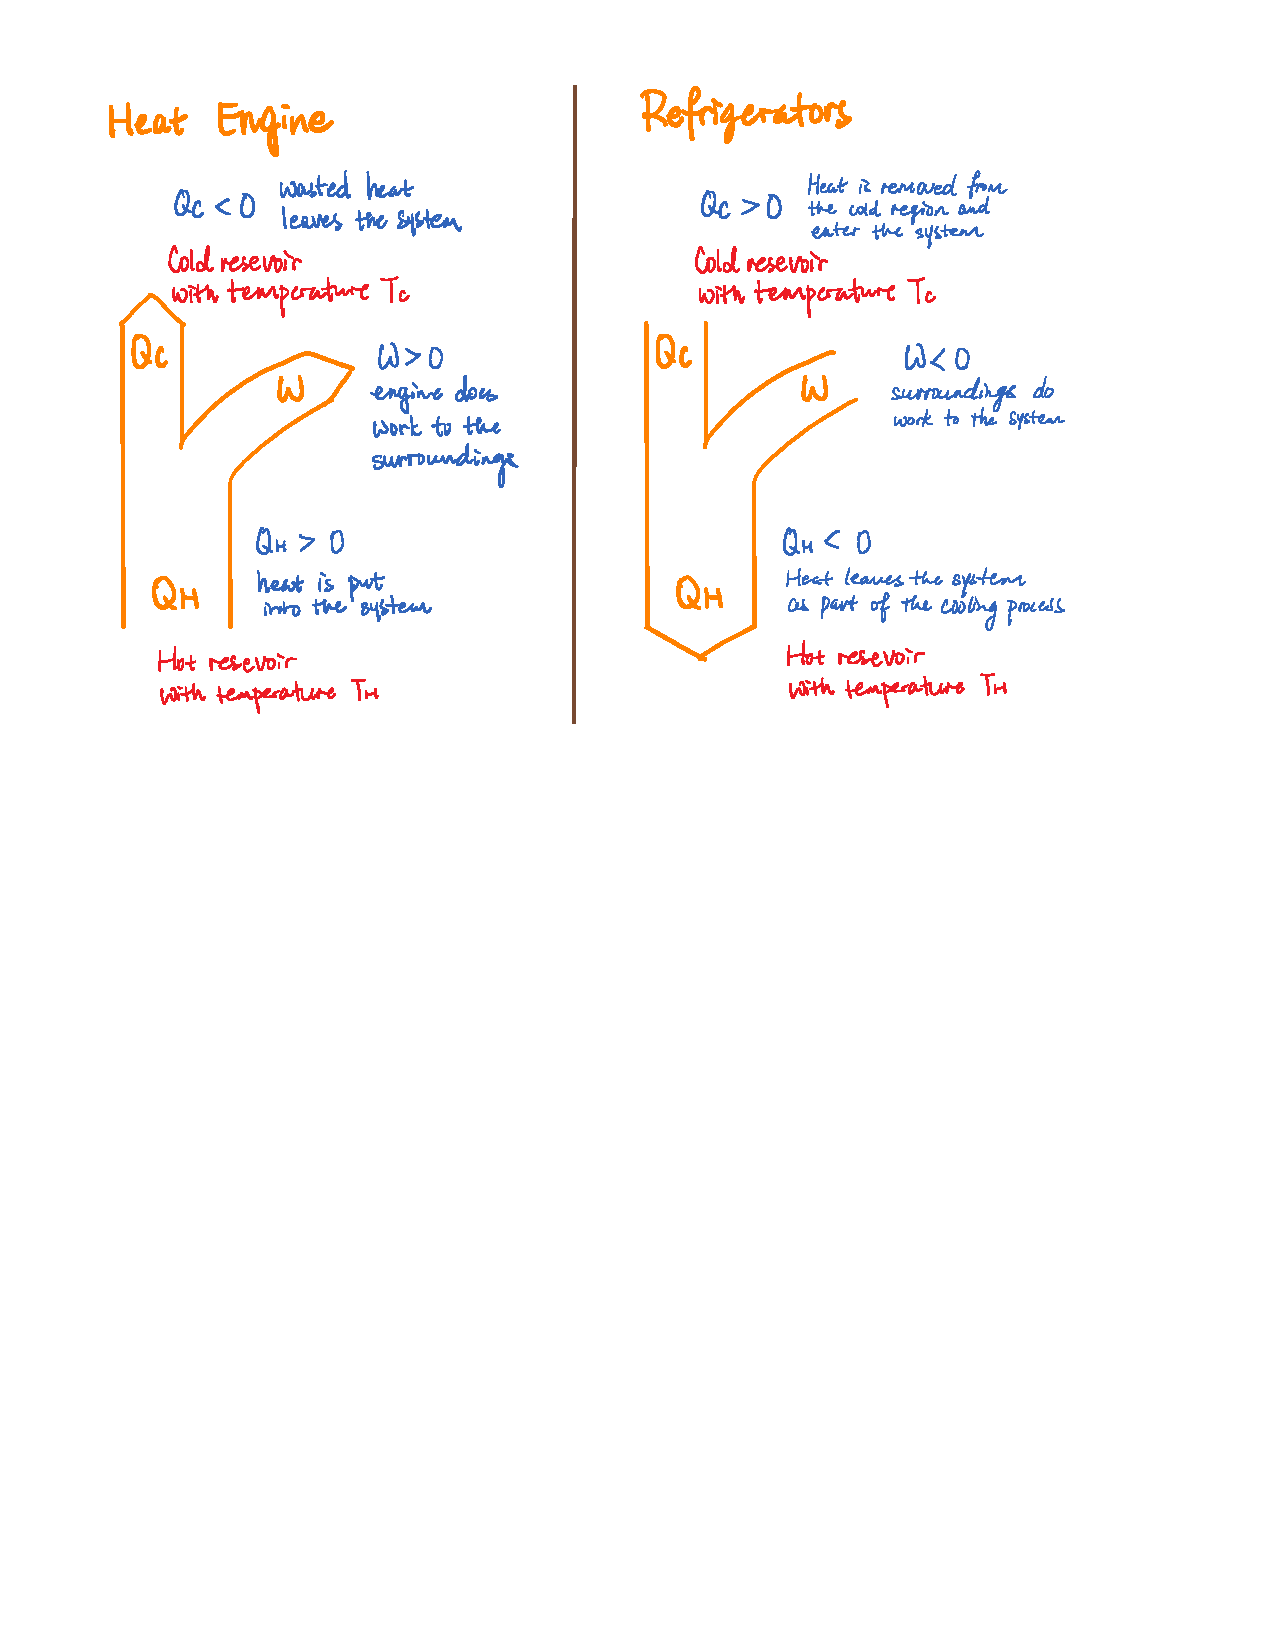
\includegraphics[scale=0.5]{cycles.pdf}
\end{center}


\end{document}
